
\subsection{Kết quả kiểm thử}
% --- Slide 2: Tổng quan ---
\begin{frame}{Tổng quan}
    \begin{itemize}
        \item Kiểm thử chức năng từng thành phần trước khi phân tích hiệu năng
        \item Các thành phần: Module cảm biến, khởi tạo hệ thống, kết nối MQTT, phát hiện té ngã, camera, xử lý hình ảnh, và cảnh báo
        \item Mục tiêu: Đảm bảo hoạt động đúng thiết kế
    \end{itemize}
\end{frame}

% --- Slide 3: Module cảm biến đeo ---
\begin{frame}[fragile]{Module cảm biến đeo (Quectel EC800K)}
    \begin{itemize}
        \item Kiểm tra: Giao tiếp AT, kết nối 4G, thu nhận GPS
        \item Quy trình: Khởi tạo UART, kiểm tra modem/SIM, đánh giá sóng, cấu hình APN, bật GPS, truy vấn tọa độ
        \item Kết quả: Hoạt động ổn định, tín hiệu mạnh (\texttt{+CSQ: 31,99}), tọa độ GPS hợp lệ
    \end{itemize}
    \begin{block}{Log tiêu biểu}
        \begin{minted}[fontsize=\footnotesize,breaklines]{text}
I (2329) SIM_4G: Received: Quectel EG800K
I (5329) SIM_4G: Received: +CSQ: 31,99
I (28339) SIM_4G: Received: +QIACT: 1,1,1,"9.204.251.200"
I (34349) SIM_4G: Received: +QGPSLOC: 10.88862,106.77975
        \end{minted}
    \end{block}
    \textbf{Kết luận:} Module 4G/GPS hoạt động đúng, hỗ trợ gửi cảnh báo và định vị.
\end{frame}

% --- Slide 4: Khởi tạo hệ thống ---
\begin{frame}[fragile]{Khởi tạo hệ thống và kết nối mạng}
    \begin{itemize}
        \item Xác nhận: Module SIM4G-GPS, Wi-Fi, và các tác vụ chính hoạt động bình thường
        \item Kết quả: Hệ thống khởi tạo thành công, tích hợp ổn định
    \end{itemize}
    \begin{block}{Log tiêu biểu}
        \begin{minted}[fontsize=\footnotesize,breaklines]{text}
I (9961) SIM4G_AT: Initializing SIM4G AT driver...
I (9981) SIM4G_AT: Successfully set APN to v-internet
I (10011) APP_MAIN: System initialization complete.
I (10021) APP_MAIN: Application started successfully
        \end{minted}
    \end{block}
    \textbf{Kết luận:} Nền tảng phần cứng và phần mềm tích hợp ổn định.
\end{frame}

% --- Slide 5: Kết nối MQTT ---
\begin{frame}[fragile]{Kết nối MQTT và truyền dữ liệu}
    \begin{itemize}
        \item ESP32 kết nối MQTT, gửi bản tin định kỳ (định danh, trạng thái té ngã, GPS)
        \item Kết quả: Kết nối ổn định, dữ liệu truyền tới hệ thống giám sát
    \end{itemize}
    \begin{block}{Log tiêu biểu}
        \begin{minted}[fontsize=\footnotesize,breaklines]{text}
I (19961) USER_MQTT: MQTT_EVENT_CONNECTED
I (39991) JSON_WRAPPER: Created status payload:
{"device_id":"ESP32_DEV_76E48B","fall_detected":false,
 "latitude":0,"longitude":0,"has_gps_fix":false}
        \end{minted}
    \end{block}
    \begin{figure}
        \centering
        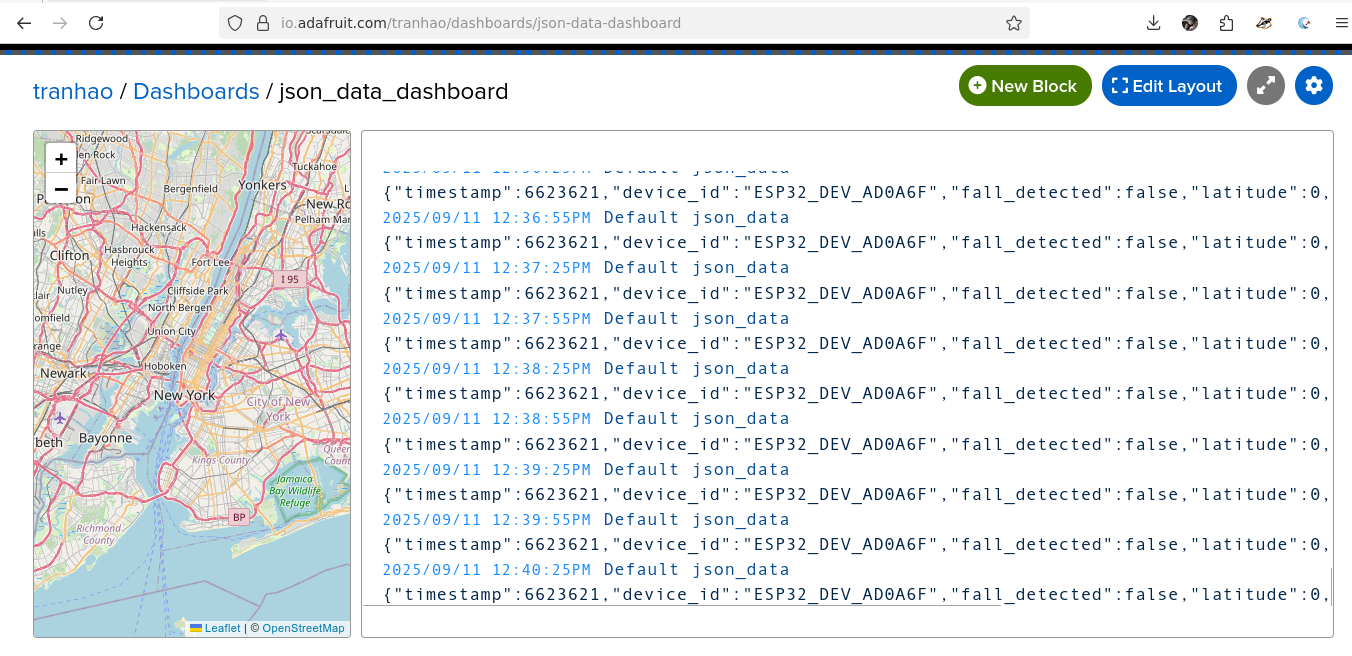
\includegraphics[width=0.6\textwidth]{images/json_data_dashboard.png}
        \caption{Dashboard hiển thị bản tin MQTT.}
    \end{figure}
\end{frame}

% --- Slide 6: Phát hiện té ngã ---
\begin{frame}[fragile]{Phát hiện té ngã và xử lý cảnh báo}
    \begin{itemize}
        \item Thuật toán: Phát hiện trạng thái \texttt{LOW_G} đến \texttt{HIGH_G}, xác nhận va chạm
        \item Cảnh báo: Gửi SMS, MQTT, kích hoạt buzzer và LED
    \end{itemize}
    \begin{block}{Log tiêu biểu}
        \begin{minted}[fontsize=\footnotesize,breaklines]{text}
E (159131) FALL_LOGIC: FALL DETECTED! Accel: 0.99 g
I (159151) SIM4G_GPS: SMS request queued successfully
I (159191) SIM4G_GPS: MQTT alert published successfully.
I (159221) buzzer: Beeping for 8000 ms
        \end{minted}
    \end{block}
    \begin{figure}
        \centering
        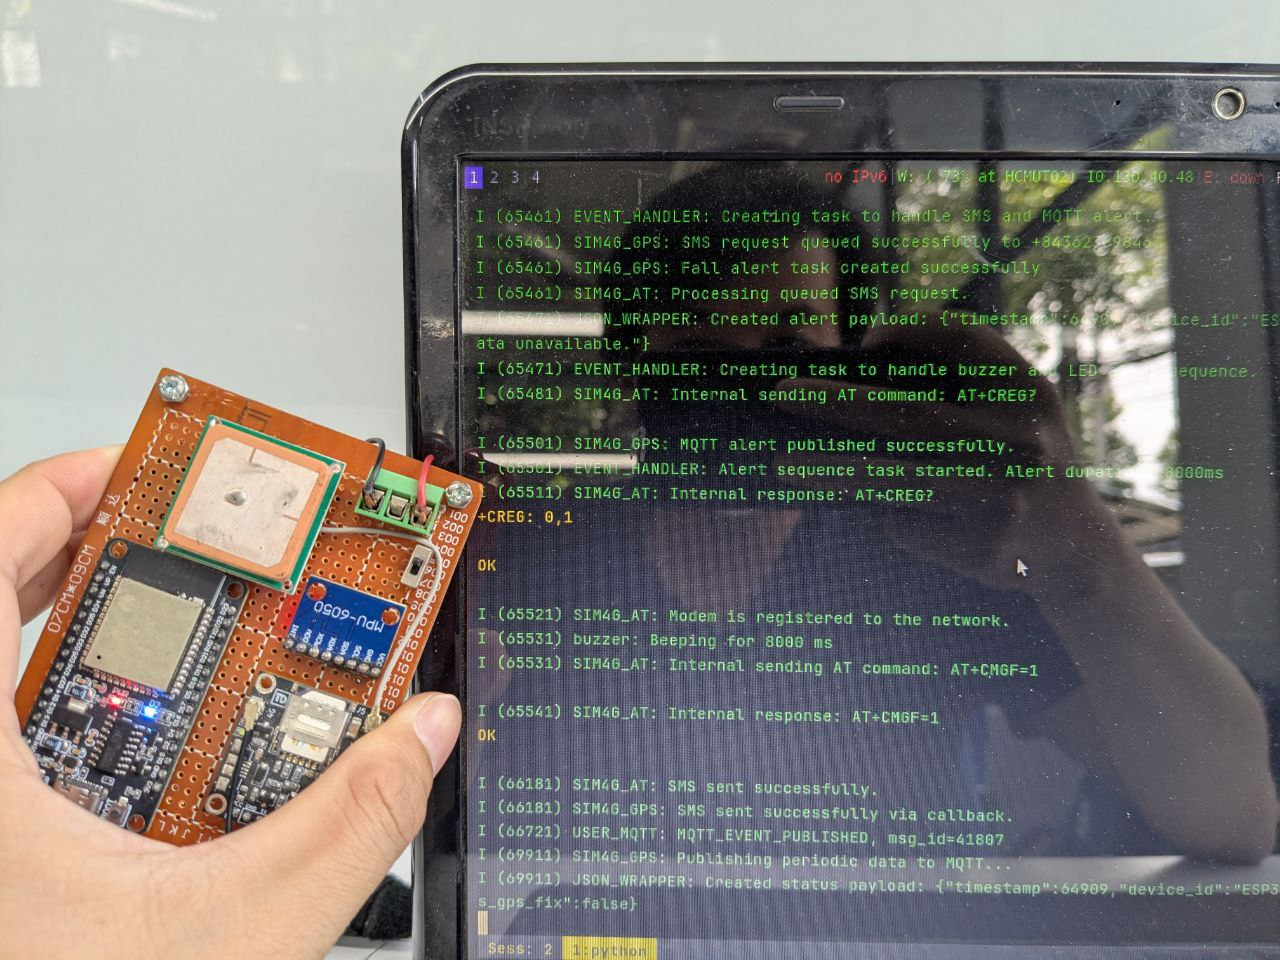
\includegraphics[width=0.6\textwidth]{images/module1_real_log.jpg}
        \caption{Log thực tế khi phát hiện té ngã.}
    \end{figure}
\end{frame}

% --- Slide 7: Module Camera ---
\begin{frame}[fragile]{Module Camera và truyền hình ảnh}
    \begin{itemize}
        \item Kiểm tra: Kết nối Wi-Fi, phát luồng HTTP (ESP32-CAM, OV5640)
        \item Kết quả: Camera nhận diện đúng, server HTTP hoạt động, FPS 3.5–5
    \end{itemize}
    \begin{block}{Log tiêu biểu}
        \begin{minted}[fontsize=\footnotesize,breaklines]{text}
I (8936) esp32cam: Got IP: 10.110.87.85
I (9266) camera: Detected OV5640 camera
I (10006) esp32cam: HTTP server started
I (20006) esp32cam: Frames sent: 50, FPS: 5.87
        \end{minted}
    \end{block}
    \begin{figure}
        \centering
        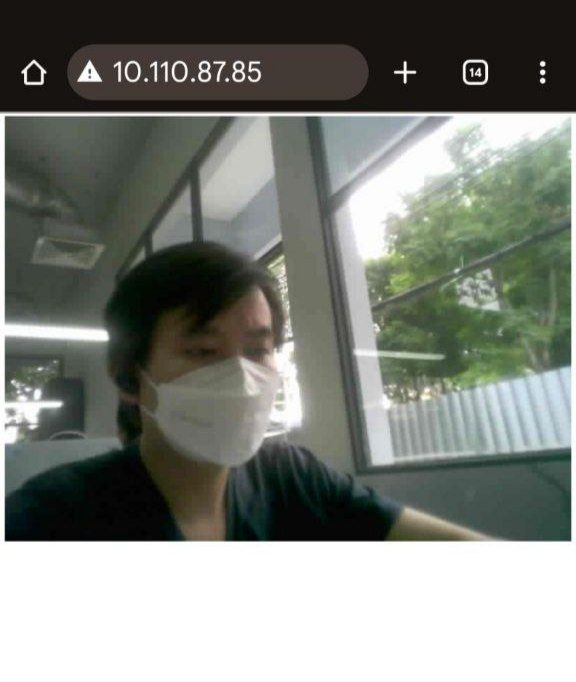
\includegraphics[width=0.6\textwidth]{images/module2_stream_example.jpg}
        \caption{Luồng hình ảnh từ ESP32-CAM.}
    \end{figure}
\end{frame}

% --- Slide 8: Xử lý hình ảnh Python - hình 1 ---
\begin{frame}{Xử lý nhận diện hình ảnh (Python)}
    \begin{itemize}
        \item Quy trình: Nhận luồng video, tiền xử lý, chạy TensorFlow Lite, vẽ skeleton
        \item Kết quả: Xử lý thời gian thực (3–5 FPS), tích hợp MQTT và Telegram
    \end{itemize}
    \begin{figure}
        \centering
        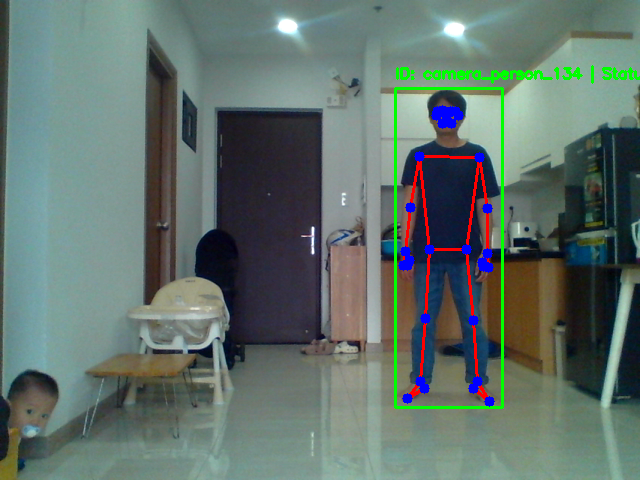
\includegraphics[width=0.7\textwidth]{images/fall_detection_screen_shoot.png}
        \caption{Phát hiện người và vẽ skeleton thời gian thực.}
    \end{figure}
\end{frame}

% --- Slide 9: Xử lý hình ảnh Python - hình 2 ---
\begin{frame}{Log xử lý ảnh Python}
    \begin{figure}
        \centering
        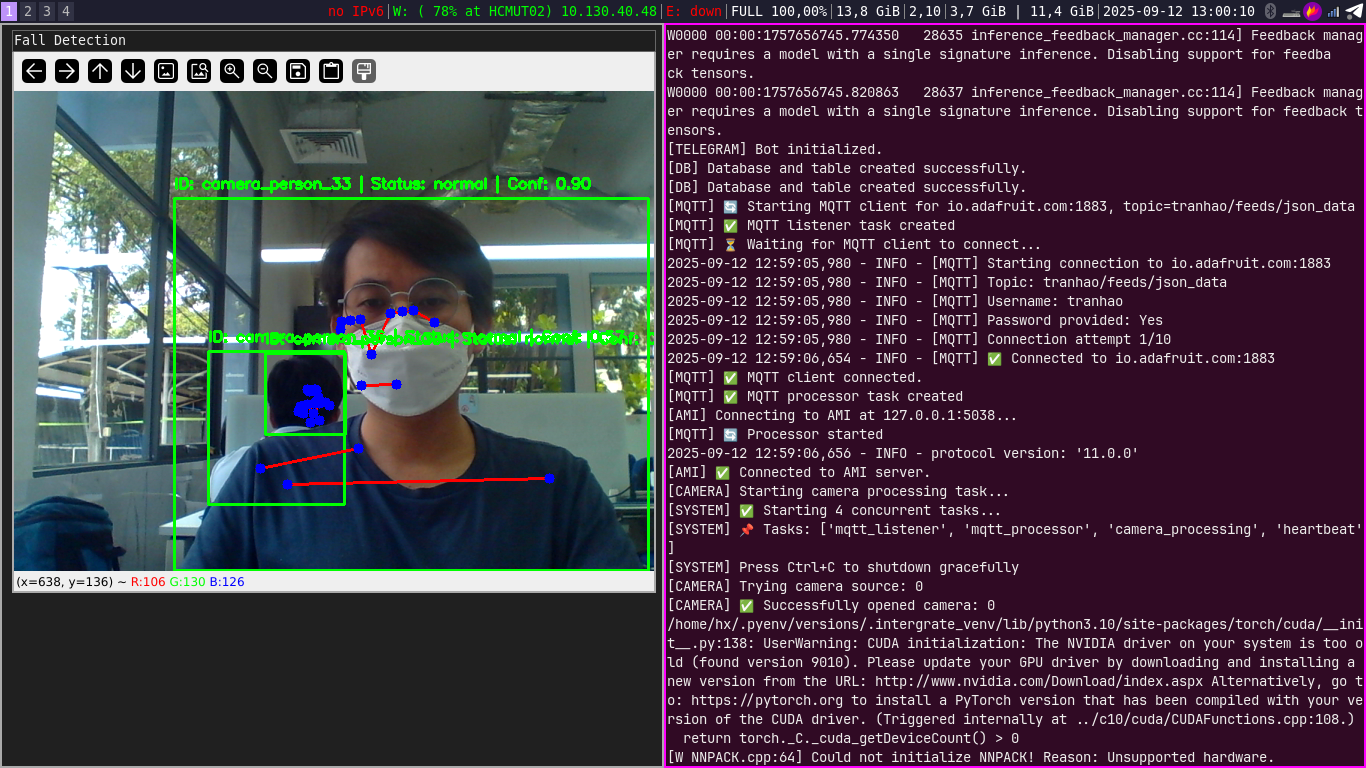
\includegraphics[width=0.7\textwidth]{images/python_runing_log.png}
        \caption{Log xử lý ảnh và điều phối tác vụ.}
    \end{figure}
\end{frame}

% --- Slide 10: Đánh giá cảm biến ---
\begin{frame}{Đánh giá thực nghiệm cảm biến MPU6050 và GPS}
    \begin{itemize}
        \item Quy trình: Nạp chương trình, giả lập té ngã, kiểm tra SMS/GPS
        \item Dữ liệu MPU6050: So sánh trạng thái bình thường và té ngã
    \end{itemize}
    \begin{table}
        \centering
        \caption{So sánh dữ liệu MPU6050}
        \begin{tabular}{|l|c|c|}
            \hline
            \textbf{Thông số} & \textbf{Bình thường} & \textbf{Té ngã} \\
            \hline
            Biên độ Gyro & $\pm 1.5$ dps & $\pm 250$ dps \\
            \hline
            Độ lớn Accel & $\approx 0.93$ g & $-2.0$ đến $+1.0$ g \\
            \hline
        \end{tabular}
    \end{table}
    \begin{figure}
        \centering
        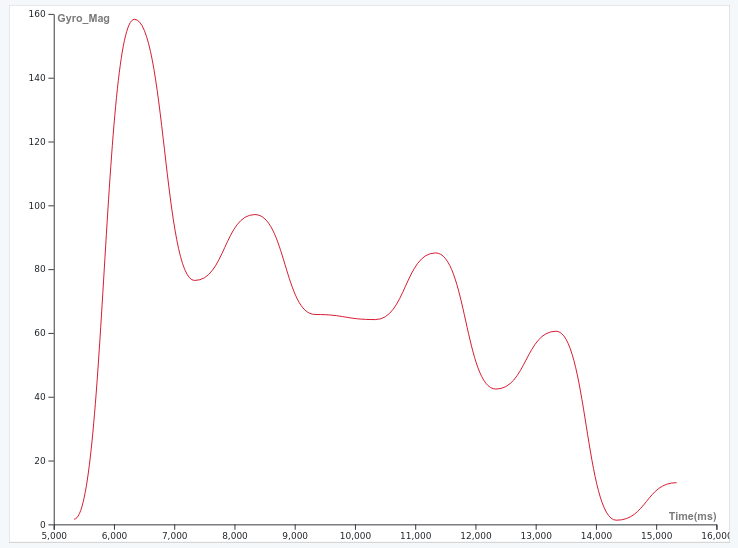
\includegraphics[width=0.6\textwidth]{images/gyro_time.png}
        \caption{Biến thiên Gyro\_Mag theo thời gian.}
    \end{figure}
\end{frame}

% --- Slide 11: Dữ liệu GPS ---
\begin{frame}{Dữ liệu GPS}
    \begin{table}
        \centering
        \caption{Dữ liệu GPS thu được}
        \begin{tabular}{|c|c|c|c|}
            \hline
            \textbf{Time (UTC)} & \textbf{Latitude} & \textbf{Longitude} & \textbf{Satellites} \\
            \hline
            132517.00 & 1053.3115N & 10646.7839E & 07 \\
            132540.00 & 1053.3117N & 10646.7840E & 07 \\
            132627.00 & 1053.3107N & 10646.7839E & 07 \\
            \hline
        \end{tabular}
    \end{table}
    \textbf{Kết luận:} GPS ổn định, định vị chính xác với 7 vệ tinh.
\end{frame}

% --- Slide 12: Thử nghiệm Asterisk ---
\begin{frame}{Thử nghiệm Asterisk AMI}
    \begin{itemize}
        \item Kiểm tra: Gửi SMS và gọi đến 3 extension (\texttt{6001}, \texttt{6002}, \texttt{6003})
        \item Kết quả: SMS thành công (2/3), lỗi gọi do thiếu nội dung thoại
    \end{itemize}
    \begin{figure}
        \centering
        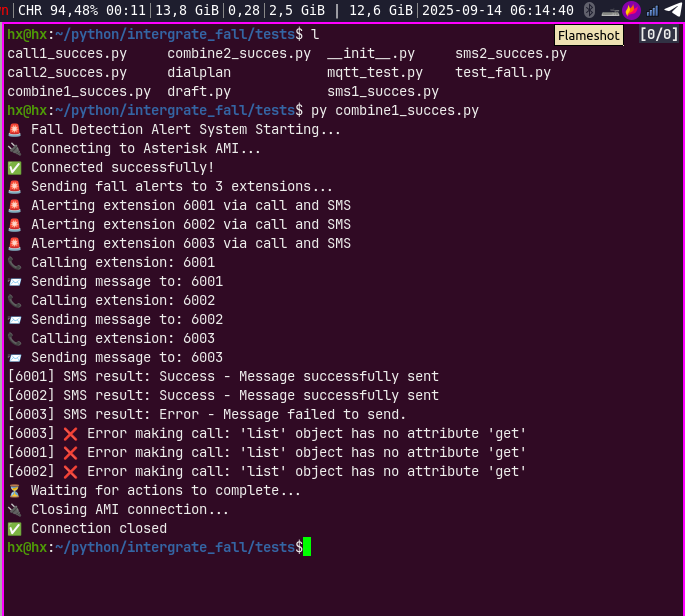
\includegraphics[width=0.6\textwidth]{images/ast_call_sms_test.png}
        \caption{Log thử nghiệm Asterisk AMI.}
    \end{figure}
    \textbf{Kết luận:} Cảnh báo SMS hoạt động, lỗi gọi không ảnh hưởng chức năng chính.
\end{frame}

% --- Slide 13: Telegram ---
\begin{frame}{Kênh cảnh báo Telegram}
    \begin{itemize}
        \item Cảnh báo từ: ESP32 (MQTT) và Python (hình ảnh + skeleton)
        \item Kết quả: Cảnh báo gửi thành công, tăng độ tin cậy
    \end{itemize}
    \begin{figure}
        \centering
        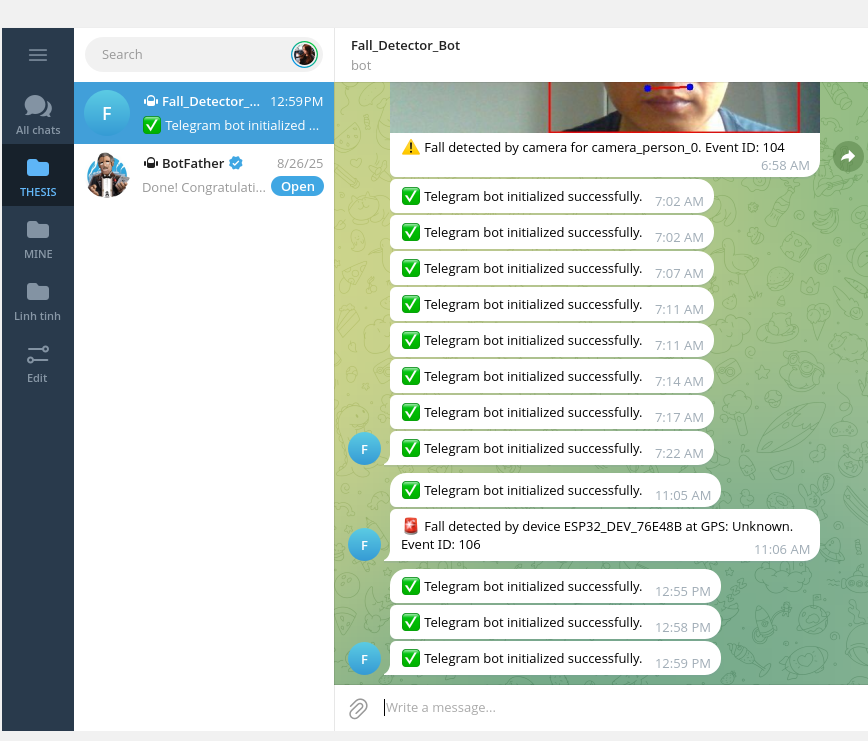
\includegraphics[width=0.6\textwidth]{images/telegram_fall_module1_send.png}
        \caption{Cảnh báo từ ESP32 qua Telegram.}
    \end{figure}
    \begin{figure}
        \centering
        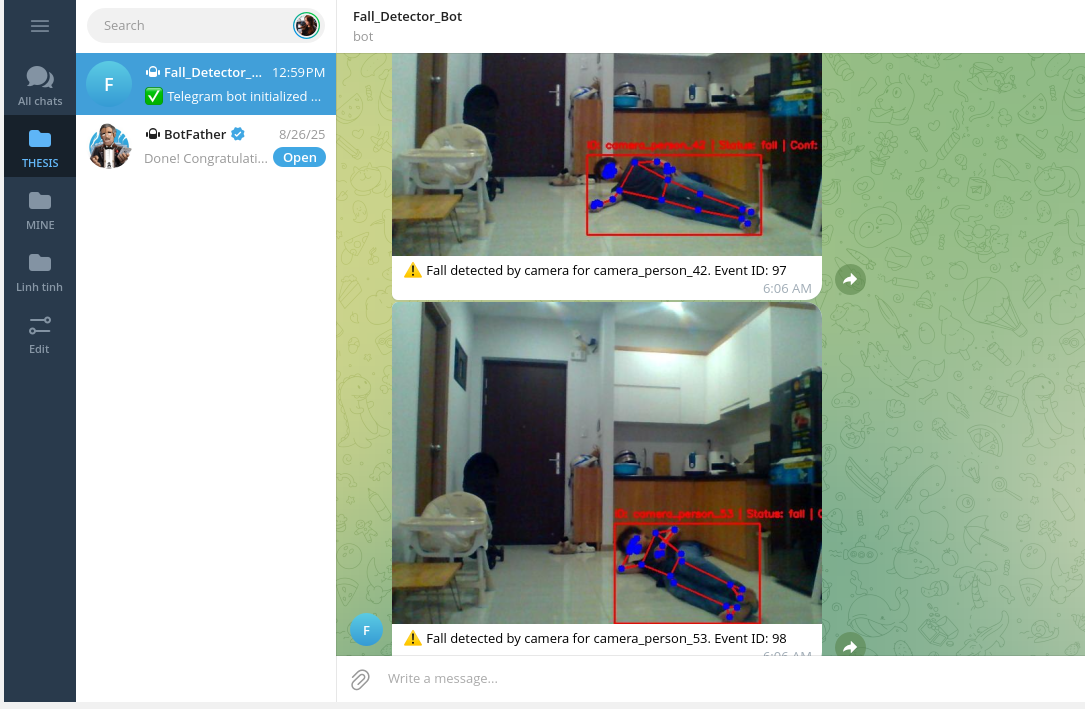
\includegraphics[width=0.6\textwidth]{images/telegram_python_fall_send.png}
        \caption{Cảnh báo từ Python qua Telegram.}
    \end{figure}
\end{frame}

% --- Slide 14: Kết luận ---
\begin{frame}{Kết luận}
    \begin{itemize}
        \item Tất cả thành phần (cảm biến, camera, MQTT, Telegram, Asterisk) hoạt động ổn định
        \item Phát hiện té ngã chính xác với dữ liệu MPU6050 và GPS
        \item Hệ thống tích hợp đa kênh cảnh báo hiệu quả
        \item Hạn chế: Lỗi gọi Asterisk (không ảnh hưởng chính), FPS camera còn thấp
    \end{itemize}
\end{frame}
